% -------------------------------------------------------
%    UMKC Thesis
%    Version 1.3
%    2012.04.17
% -------------------------------------------------------


\documentclass[12pt]{sty/myreport}


\newcommand{\MyThesisTitle}{My Thesis Title: As I See This World: 
To Try Out a Very Long Title So that We can Check This Out}

% student's name
\newcommand{\MyName}{Jane Doe}

%  change to appropriate school or college
\newcommand{\MyUMKCSchool}{School of Computing and Engineering}

% degree award year for this degree
\newcommand{\MyDegreeAwardYear}{2012}

% change the degree title to Maser of Arts, if applicable in your case
\newcommand{\MyDegree}{Master of Science}



% for MS thesis use the following tag format:
\newcommand{\MyField}{Computer Science}
\newcommand\ThesisOrDissertation{Thesis}

% for i-PhD dissertation that requires two disciplines, 
%   use the following tag format for MyField
%   and uncomment all of the following
%
% \renewcommand{\MyField}{Telecommunications and Computer Networking\\ and\\ Mathematics}
% \renewcommand\ThesisOrDissertation{Dissertation}
% \renewcommand{\MyDegree}{Doctor of Philosophy}
% \renewcommand{\MyUMKCSchool}{School of Graduate Studies}



%\def\figureref#1{Fig.~\ref{#1}}
%\def\figref#1{Fig.~\ref{#1}}
%\def\tableref#1{Table~\ref{#1}}
% -------------------------------------------------------

\usepackage[latin1]{inputenc}
\usepackage{times, indentfirst, ulem, array, cite, url, rotate}
\usepackage{epsf, rotate, url}
\usepackage{amssymb, amsfonts, amsthm, subeqn}
\usepackage{graphicx}
\usepackage{sty/mysymbols}
\usepackage{sty/umkc-thesis} % UMKC thesis style file umkc-thesis.sty
\usepackage{sty/umkc-tocinc} % Include Table of Contents as the first entry in TOC


% file:    Defns-LQE.tex
% date:    July 27, 2005
% author:  Larry Eifler
%


\def\singlespace{\baselineskip=12pt\relax}                                             

\def\text#1{\mbox{#1}}  %  Poor man's \text  

% Declarations for theorem-like structures

\newtheorem{theorem}{THEOREM}[chapter]
\newtheorem{lemma}[theorem]{LEMMA} 
\newtheorem{proposition}[theorem]{PROPOSITION} 
\newtheorem{definition}[theorem]{DEFINITION} 
\newtheorem{corollary}[theorem]{COROLLARY}
\newtheorem{remark}[theorem]{REMARK}
\newtheorem{example}[theorem]{EXAMPLE} 

\def\proof{\trivlist %
   \item[\hskip \labelsep{PROOF.\quad}]}

\def\QEDmark{\null\hfill \makebox{$\sqcup\hskip-8pt\sqcap$} }
\def\endproof{\QEDmark\endtrivlist}   %  Ends proof with a marker.

\font\BlackBoard msbm10 at 12pt \relax
\def\Bbb#1{\mbox{\BlackBoard #1}} 

\newcommand{\BbR}{\mbox{\BlackBoard R}}
\newcommand{\BbN}{\mbox{\BlackBoard N}}
\newcommand{\BbC}{\mbox{\BlackBoard C}}
\newcommand{\BbZ}{\mbox{\BlackBoard Z}}
\newcommand{\BbQ}{\mbox{\BlackBoard Q}}
\newcommand{\BbK}{\mbox{\BlackBoard K}}
\newcommand{\BbH}{\mbox{\BlackBoard H}}
\newcommand{\BbD}{\mbox{\BlackBoard D}}

\endinput




\setlength{\baselineskip}{26pt}

\setcounter{page}{1}

\begin{document}


%%%%%%%%%%%%%%%%%%%%%%%%%%%%%%%%%%%%%%%%%%%%%%%%%%%%%%%%%%%%%%%%%%%%%%%%%%
% Title page goes here
\thispagestyle{empty}   %no number on the title page

\setlength{\baselineskip}{28pt}

% file:    TitlePage-LQE.tex
% date:    July 27, 2005
% author:  Larry Eifler 
%    


\typeout{TITLE PAGE}

%\setlength{\topsep}{0pt}  
\setcounter{page}{0}    
\pagenumbering{roman}

\thispagestyle{empty}
\null\vspace{-12pt}    
%
\begin{center}
\singlespace
     A TEMPLATE USING LATEX FOR DISSERTATIONS \\[1pc]  % 1pc = 12pt
     IN MATHEMATICS VERSION 10/28/2005


\vspace{9.2pc}   % subtract  2pc  for extra line in title  


     A DISSERTATION IN \\
     Mathematics \\
      and        \\
     ``Co-Discipline''   \\[1pc]

     Presented to the Faculty of the University \\
     of Missouri-Kansas City in partial fulfillment of \\
     the requirements for the degree \\[1pc]

     DOCTOR OF PHILOSOPHY
\end{center}

\vspace{6.0pc}    %  the center environment adds \topsep=12pt
                  %  to the space above and below

\begin{center}
\singlespace
     by \\
     LARRY QUIN EIFLER \\[1pc]

     B.S., University of Missouri-Kansas City, 1964 \\
     M.S., Purdue University, 1966
\end{center}

\vspace{5.1pc}

\begin{center}
\singlespace
     Kansas City, Missouri \\
     2005
\end{center}


\newpage

\pagestyle{plain}

%% -- A blank page or copyright blank goes here.
%% -- A blank page can be printed using:  {  } \newpage

\thispagestyle{empty}
\vspace*{36pc}
\begin{center}
      \copyright\ 2005    \\
      LARRY QUIN EIFLER   \\
      ALL RIGHTS RESERVED 
\end{center}
\newpage

\endinput


\pagebreak

%%%%%%%%%%%%%%%%%%%%%%%%%%%%%%%%%%%%%%%%%%%%%%%%%%%%%%%%%%%%%%%%%%%%%%%%%%
% Copyright page goes here
\thispagestyle{empty}   %no number on the title page
%%%%
%   This is the copyright page
%%%%
%--------------------------------------------------------------------------
\vspace*{6in}
\begin{center}
\normalsize{
\copyright \hspace{0.02in} \MyDegreeAwardYear

\MakeUppercase{\MyName}

ALL RIGHTS RESERVED
}
\end{center}
%--------------------------------------------------------------------------

\pagebreak

%%%%%%%%%%%%%%%%%%%%%%%%%%%%%%%%%%%%%%%%%%%%%%%%%%%%%%%%%%%%%%%%%%%%%%%%%%
% Abstract page goes here
\pagenumbering{roman}
\setcounter{page}{3}
\pagestyle{plain}   %puts page number at bottom-center
\setlength{\baselineskip}{26pt}

%%
%  This file contains the abstract of the dissertation
%%
%----------------------------------------------------------------------------
\begin{center}
\vspace*{0.01in}
\MakeUppercase{\MyThesisTitle}\\


\vspace{24pt}
\MyName, Candidate for the \MyDegree\ Degree\\
University of Missouri--Kansas City, \MyDegreeAwardYear\\
\vspace{24pt}
ABSTRACT
\vspace{24pt}
\end{center}
\addcontentsline{toc}{chapter}{ABSTRACT}  %the name 'ABSTRACT' will appear in the toc, as a chapter
\doublespacing


Here is my abstract -- It is short. Please make me the right size to meet the requirement. It seems it is no longer
required include the length of the abstract in word count. and uncomment in the LaTeX source file for abstract. 

\comment{
\vspace{25pt}
This abstract of NNN words is approved as to form
and content.
\vspace{20pt}
\begin{flushright}
    \underline{\hspace{11cm}}\\
    \singlespacing
    Advisor's Name, Ph.D.\\
        Professor\\
        Department of Computer Science \& Electrical Engineering
%    School of Computing and Engineering
\end{flushright}
}
% \newpage
% \quad \thispagestyle{empty}
%----------------------------------------------------------------------------

\pagebreak


%%%%%%%%%%%%%%%%%%%%%%%%%%%%%%%%%%%%%%%%%%%%%%%%%%%%%%%%%%%%%%%%%%%%%%%%%%
% Approval page goes here
%\thispagestyle{empty} % not numbered (but counted)

%%%
%  This is the approval page
%%%
%-----------------------------------------------------------------------------------
%\thispagestyle{empty}

\begin{center}
   \MakeUppercase{Approval Page}
\end{center}
 \setlength{\baselineskip}{24pt}
The faculty listed below, appointed by the Dean of the \MyUMKCSchool,
 have examined a \MakeLowercase{\ThesisOrDissertation}\ titled
``\MyThesisTitle,''
presented by \MyName, candidate
for the \MyDegree\ degree, and hereby certify that in
their opinion it is worthy of acceptance.

\vspace{0.3in}
\setlength{\baselineskip}{5pt}
%\singlespacing

\begin{center}
\underline{Supervisory Committee}\\
\vspace{0.25in}
Advisor Name, Ph.D., Committee Chair\\
Department of Computer Science \& Electrical Engineering\\

\vspace{0.25in}
Committee Member Name-1, Ph.D.\\
Department of Computer Science \& Electrical Engineering\\
\vspace{0.25in}
Committee Member Name-2, Ph.D.\\
Department of Computer Science \& Electrical Engineering\\

\end{center}

%-----------------------------------------------------------------------------------
\newpage
 \thispagestyle{empty}

\setlength{\baselineskip}{26pt}
\pagebreak


%%%%%%%%%%%%%%%%%%%%%%%%%
%  Table of content

\tableofcontents

% List of Figures
\listoffigures 
   
% List of Tables

\listoftables
\pagebreak

%  
% If your thesis/dissertation has a list of acronyms,
% you can uncomment the following; be sure to include your list
% in acronym.tex

% \pagestyle{plain}   %puts page number at bottom-center
% \addcontentsline{toc}{chapter}{ACRONYMS}
% \include{./acronym}
% \pagebreak


% Acknowledgement page goes here
\thispagestyle{empty}
\addcontentsline{toc}{chapter}{ACKNOWLEDGEMENTS}
\addtocontents{toc}{\noindent Chapter}
%%%%
%%  This is the acknowledgement page
%%%%
%--------------------------------------------------------------
\begin{center}
\vspace*{0.01in}
ACKNOWLEDGEMENTS
\end{center}

I would like to thank my academic advisor ...


I would like to thank my family for making this possible. 


%--------------------------------------------------------------

\pagebreak

\def\ArchName{SiDR\xspace}
%%%%%%%%%%%%%%%%%%%%%%%%%%%%%%%%%%%%%%%%%%%%%%%%%%%%%%%%%%%%%%%%%%%%%%%%%%
% Content
\setlength{\baselineskip}{26pt}

% 
\pagenumbering{arabic}  %use Arabic numbers for the rest of the diss.
\setcounter{page}{1}    %restart page numbers at one in the main text of diss.
%\pagestyle{myheadings}  %reset the page numbering to upper-right corner

%%%---------Chapter One------------------------

\chapter{INTRODUCTION}


Internet was designed for transmitting data  from point A to point B as a best effort scheme. After almost 40 years, the core design of the Internet remains the same, but the demands of the Internet usage have been drastically changed. Future Internet design is a hot area of research today as researchers try to understand the dynamics and demands of todays' Internet and predict the demands of future Internet thereby proposing novel framework and protocols that meet those demands. 
Today Internet relies heavily on the inter-domain routing to make communications happen on the Internet. The most popular inter-domain routing protocol is the Border Gateway Protocol. Another protocol in  the Asynchronous Transfer Mode (ATM) world is Private Network-to-Network Interface (PNNI). PNNI is a hierarchical state-of-art routing protocol and is known to use Quality-of-Service sensitive routing scheme by advertising topology state parameters and Call Admission Control \cite{pnni} .



\section{Section Header}

You can now see the section header, with this citation  \cite{bgpLSurvey}. 


\subsection{Subsection Header}

At the heart of the Internet lies routing.  This shows your subsection header.


\subsubsection{Subsection Header}

Do you really want subsubsection header? This is not recommended in a thesis or dissertation.


\section{Summary of Contributions}

The main contributions of this work are as follows:

  \begin{itemize}

    \item A new model is proposed to do ...
    \item A new algorithm is proposed to solve the model ...
   
  \end{itemize}


%%%---------Chapter Two------------------------

\chapter{\uppercase{Real Good Stuff}}


In this chapter, I have the following figures:

%%%----------------------------------------------------------------------
\begin{figure}
  % Requires \usepackage{graphicx}
  \center
  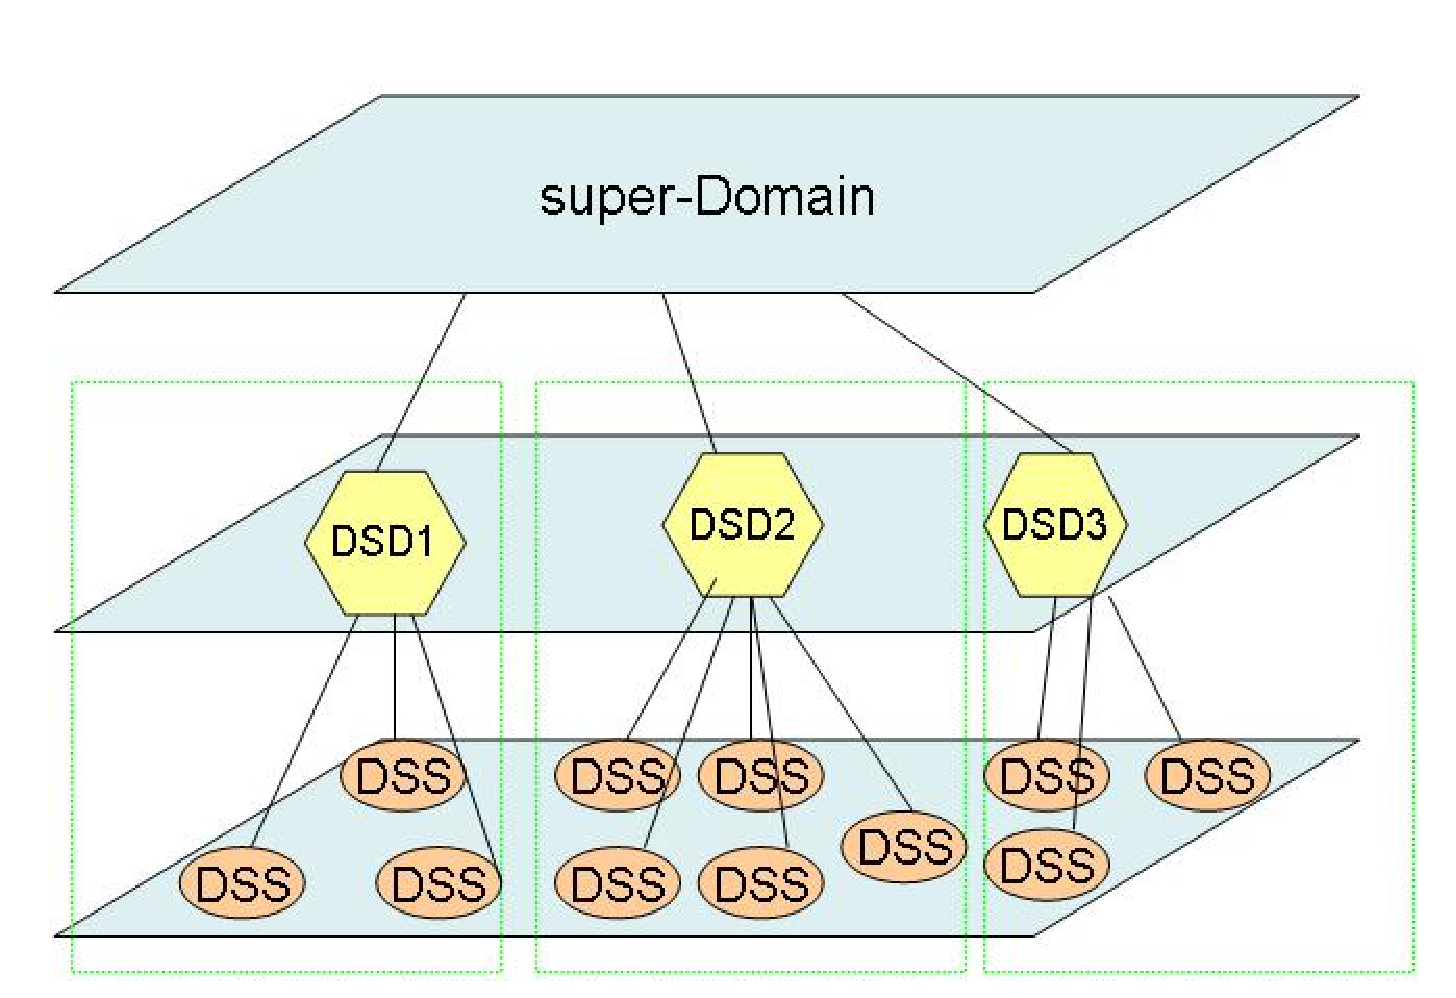
\includegraphics[scale=0.3]{figures/arch.eps}
  \caption{High level architecture}\label{chap2:fig1}
\end{figure}
%%%-----------------------------------------------------------------------


%%%----------------------------------------------------------------------
\begin{figure}
  % Requires \usepackage{graphicx}
  \center
  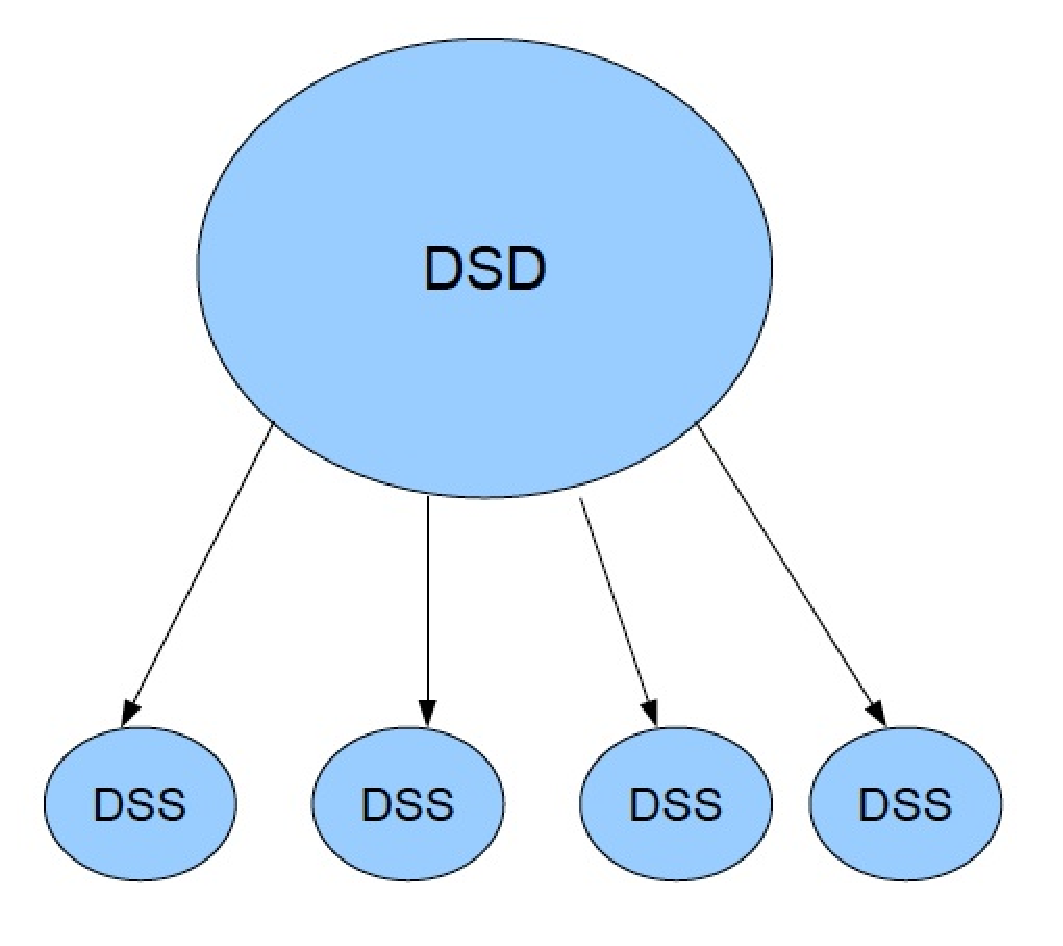
\includegraphics[scale=0.3]{figures/DSDDSS.eps}
  \caption{Relationship between a DSD and DSS}\label{chap2:fig2}
\end{figure}
%%%-----------------------------------------------------------------------


\figureref{chap2:fig1}  shows the high level routing structure of SiDR. 
\figureref{chap2:fig2} shows the relationship between a DSD and a DSS. 



%%%---------Chapter Three------------------------

\chapter{Table}

This chapter includes a table. This table is shown as \tableref{tab:otn}.

\begin{table}[!t]
\renewcommand{\arraystretch}{1.1}
\caption{OTN Signals, Data Rates and Multiplexing.}
\label{tab:otn}
\centering
\begin{tabular}{c|c|c}
\hline
$U_{k}$ Signal &  Bit-Rate (Gbps) & Max. $U_{k}$s in a wavelength\\
\hline
$U_{0}$ & 1.25  & 80 \\
$U_{1}$ & 2.5  & 40 \\
$U_{2}$ & 10 & 10\\
$U_{3}$ & 40 & 2\\
$U_{4}$ & 100 & 1\\
\hline
\end{tabular}
\end{table}


\begin{table}[!t]
\renewcommand{\arraystretch}{1.1}
\caption{OTN Signals, Data Rates and Multiplexing -- 2nd table.}
\label{tab:otn2}
\centering
\begin{tabular}{c|c|c}
\hline
$U_{k}$ \textbf{Signal} &  Bit-Rate (Gbps) & Max. $U_{k}$s in a wavelength\\
\hline
$U_{0}$ & 1.25  & 80 \\
$U_{1}$ & 2.5  & 40 \\
$U_{2}$ & 10 & 10\\
$U_{3}$ & 40 & 2\\
$U_{4}$ & 100 & 1\\
\hline
\end{tabular}
\end{table}





%%%-------and so on for as many chapters as you want ------------------------


%% +++ Appendix  %%

%% Somehow this abnormal placement produces the desired output
\addtocontents{toc}{\noindent Appendix}

%%%%%%%%%%%%%%%%%%%%%%%%%%%%%%%%%%%%%%%%%%%%%%%%%%%%%%%%%%%%%%%%%%%%%%%%%%%

\appendix
\chapter{Information }

This is an appendix.


Just a place holder this is created.




%%%%%%%


% you don't want to activate \nocite unless you want all references
% from your bibfile to show up

% \nocite{*}

\def\uline#1{{\it #1}}

% acm style is used by School of Computing and Engineering at UMKC
% Please active an appropriate style file for your school/department

\bibliographystyle{sty/myacm}

% here are the rest; however, they haven't been tested to see they conform to UMKC requirements
% \bibliographystyle{./../sty/acs}        %%%% ACS
% \bibliographystyle{./../sty/apa}        %%%% APA
% \bibliographystyle{./../sty/phaip}      %%%% AIP
% \bibliographystyle{./../sty/chicago}    %%%% Turabian

\bibliography{biblio/references}

%%%%%%%%%%%%%%%%%%%%%%%%%%%%%%%%%%%%%%%%%%%%%%%%%%%%%%%%%%%%%%%%%%%%%%%%%%%
\thispagestyle{empty} \addcontentsline{toc}{chapter}{VITA}
 % \addtocontents{toc}{\noindent VITA}
% file:    Vita-LQE.tex
% date:    July 27, 2005
% author:  Larry Eifler 
%    


\chapter*{VITA}
\addcontentsline{toc}{chapter}{VITA}

     Larry Quin Eifler was born on March 13, 1943, 
in Independence, Kansas.  In 1960 he graduated 
from Paseo High School in Kansas City, Missouri.
He received a B.S. degree from the 
University of Missouri-Kansas City in 1964.

\clearpage
\endinput

%%%%%%%%%%%%%%%%%%%%%%%%%%%%%%%%%%%%%%%%%%%%%%%%%%%%%%%%%%%%%%%%%%%%%%%%%%%

\end{document}
